 \documentclass[a4paper,11pt]{article}
\usepackage{fullpage}
\usepackage{amsmath}
\usepackage[boxed]{algorithm}   % drop [boxed] is no box around algorithm wanted
\usepackage[noend]{algorithmic} % drop [noend] if endif, endwhile, etc wanted
\renewcommand{\algorithmiccomment}[1]{\hfill // #1}
\usepackage{graphicx}
\usepackage{listings}
\usepackage{tikz}

\lstdefinelanguage{Python}{
keywords={typeof, null, catch, switch, in, int, str, float, self},
keywordstyle=\color{ForestGreen}\bfseries,
ndkeywords={return,class,if,elif,endif,while, do, else, True, False, def},
ndkeywordstyle=\color{BrickRed}\bfseries,
identifierstyle=\color{black},
sensitive =false,
comment=[1]{\#}
commentstyle=\color{purple}\ttfamily,
stringstyle=\color{red}\ttfamily,
}


\usepackage[
    backend=biber,
    style=ieee,
    sorting=nyt,
    autolang=other
]{biblatex}
\title{\textbf{Software Testing of \\ Numpy Linear Algebra Library\\
        by Team~$7$                                   % Replace t by team number
}
}

\author{Regina \and Suraj \and Johan}  % Replace by your name(s)

    \date{\today}

    \renewcommand{\thesubsection}{\thesection.\Alph{subsection}}


\begin{document}
	
	%\tableofcontents 
	
\section{Black-box Testing}
\subsection{linalg.dot}
\subsubsection{documentation}
For 2-D arrays it is equivalent to matrix multiplication, and for 1-D arrays to inner product of vectors (without complex conjugation). For N dimensions it is a sum product over the last axis of a and the second-to-last of b:

    dot(a, b)[i,j,k,m] = sum(a[i,j,:] * b[k,:,m])
   \paragraph{Paramaters}: two arrays a: array\_like First argument.\\
b : array\_like Second argument.\\
out : ndarray, optional output argument. This must have the exact kind that would be returned if it was not used. In particular, it must have the right type, must be C-contiguous, and its dtype must be the dtype that would be returned for dot(a,b). This is a performance feature. Therefore, if these conditions are not met, an exception is raised, instead of attempting to be flexible.
    \paragraph{Returns}:    output : ndarray\\
Returns the dot product of a and b. If a and b are both scalars or both 1-D arrays then a scalar is returned; otherwise an array is returned. If out is given, then it is returned.
Raises: 
ValueError
If the last dimension of a is not the same size as the second-to-last dimension of b.


\subsubsection{tests}


\subsection{linalg.multidot}
Compute the dot product of two or more arrays in a single function call, while automatically selecting the fastest evaluation order.

multi\_dot chains numpy.dot and uses optimal parenthesization of the matrices [R44] [R45]. Depending on the shapes of the matrices, this can speed up the multiplication a lot.

If the first argument is 1-D it is treated as a row vector. If the last argument is 1-D it is treated as a column vector. The other arguments must be 2-D.
\subsubsection{tests}

\subsection{linalg.vdot}

\subsubsection{documentation}
Return the dot product of two vectors.

The vdot(a, b) function handles complex numbers differently than dot(a, b). If the first argument is complex the complex conjugate of the first argument is used for the calculation of the dot product.

Note that vdot handles multidimensional arrays differently than dot: it does not perform a matrix product, but flattens input arguments to 1-D vectors first. Consequently, it should only be used for vectors.
\subsubsection{tests}

\subsection{linalg.inner}
\subsubsection{documentation}
Inner product of two arrays.

Ordinary inner product of vectors for 1-D arrays (without complex conjugation), in higher dimensions a sum product over the last axes.

\subsubsection{tests}
\subsection{linalg.outer}
\subsubsection{documentation}
Compute the outer product of two vectors.

\paragraph{Paramaters}: 
a : (M,) array\_like
First input vector. Input is flattened if not already 1-dimensional.
b : (N,) array\_like
Second input vector. Input is flattened if not already 1-dimensional.\\
out : (M, N) ndarray, optional
A location where the result is stored\\
\paragraph{Returns}:    
out : (M, N) ndarray
out[i, j] = a[i] * b[j]

\subsubsection{tests}

\subsection{linalg.matmul}
\subsubsection{documentation}
Matrix product of two arrays.\\

The behavior depends on the arguments in the following way.\\

If both arguments are 2-D they are multiplied like conventional matrices.\\
If either argument is N-D, N > 2, it is treated as a stack of matrices residing in the last two indexes and broadcast accordingly.\\
If the first argument is 1-D, it is promoted to a matrix by prepending a 1 to its dimensions. After matrix multiplication the prepended 1 is removed.\\
If the second argument is 1-D, it is promoted to a matrix by appending a 1 to its dimensions. After matrix multiplication the appended 1 is removed.\\
Multiplication by a scalar is not allowed, use * instead. Note that multiplying a stack of matrices with a vector will result in a stack of vectors, but matmul will not recognize it as such.\\

\subsubsection{tests}
\subsection{linalg.tensordot}
\subsubsection{documentation}
Compute tensor dot product along specified axes for arrays >= 1-D.

Given two tensors (arrays of dimension greater than or equal to one), a and b, and an array\_like object containing two array\_like objects, (a\_axes, b\_axes), sum the products of a‘s and b‘s elements (components) over the axes specified by a\_axes and b\_axes. The third argument can be a single non-negative integer\_like scalar, N; if it is such, then the last N dimensions of a and the first N dimensions of b are summed over.

\subsubsection{tests}
%\subsection{linalg.einsum}
%\subsubsection{documentation}


%\subsubsection{tests}
\subsection{linalg.matrix\_power}
\subsubsection{documentation}
Raise a square matrix to the (integer) power n.\\

For positive integers n, the power is computed by repeated matrix squarings and matrix multiplications. If n == 0, the identity matrix of the same shape as M is returned. If n < 0, the inverse is computed and then raised to the abs(n).
\subsubsection{tests}
%\subsection{linalg.kron}
%\subsubsection{documentation}


%\subsubsection{tests}
\subsection{linalg.eig}
Compute the eigenvalues and right eigenvectors of a square array.
\paragraph{Paramaters}: 
a : (..., M, M) array\\
\paragraph{Returns}:    
w : (..., M) array\\
Raises: 
LinAlgError
If the eigenvalue computation does not converge.

\subsubsection{documentation}
\subsubsection{tests}
\subsection{linalg.eigh}

\subsubsection{documentation}
Return the eigenvalues and eigenvectors of a Hermitian or symmetric matrix.

Returns two objects, a 1-D array containing the eigenvalues of a, and a 2-D square array or matrix (depending on the input type) of the corresponding eigenvectors (in columns).
\paragraph{Paramaters}: 
a : (..., M, M) array\\
\paragraph{Returns}:    
w : (..., M) ndarray
The eigenvalues in ascending order, each repeated according to its multiplicity.\\
Raises: 
LinAlgError
If the eigenvalue computation does not converge.\\



\subsubsection{tests}
\subsection{linalg.eigvalsh}
\subsubsection{documentation}
Compute the eigenvalues of a Hermitian or real symmetric matrix.

Main difference from eigh: the eigenvectors are not computed.
\paragraph{Paramaters}: 
a : (..., M, M) array\_like\\
\paragraph{Returns}:    
w : (..., M,) ndarray
The eigenvaues in ascending order, each repeated according to its multiplicity.\\
Raises: 
LinAlgError if the eigenvalue computation does not converge.

\subsubsection{tests}
\subsection{linalg.eigvals}
\subsubsection{documentation}
Compute the eigenvalues of a general matrix.

Main difference between eigvals and eig: the eigenvectors aren’t returned.


\paragraph{Paramaters}: 
a : (..., M, M) array\_like
A complex- or real-valued matrix whose eigenvalues will be computed.\\
\paragraph{Returns}:    
w : (..., M,) ndarray
The eigenvalues, each repeated according to its multiplicity. They are not necessarily ordered, nor are they necessarily real for real matrices.\\
Raises: 
LinAlgError
If the eigenvalue computation does not converge.\\
\subsubsection{tests}
\subsection{linalg.norm}
\subsubsection{documentation}
Matrix or vector norm.

This function is able to return one of eight different matrix norms, or one of an infinite number of vector norms (described below), depending on the value of the ord parameter.\\

\paragraph{Paramaters}: 
x : array\_like
Input array. If axis is None, x must be 1-D or 2-D.
ord : {non-zero int, inf, -inf, ‘fro’, ‘nuc’}, optional
Order of the norm (see table under Notes). inf means numpy’s inf object.
axis : {int, 2-tuple of ints, None}, optional
If axis is an integer, it specifies the axis of x along which to compute the vector norms. If axis is a 2-tuple, it specifies the axes that hold 2-D matrices, and the matrix norms of these matrices are computed. If axis is None then either a vector norm (when x is 1-D) or a matrix norm (when x is 2-D) is returned.
keepdims : bool, optional
If this is set to True, the axes which are normed over are left in the result as dimensions with size one. With this option the result will broadcast correctly against the original x.
New in version 1.10.0.\\

\paragraph{Returns}:    
n : float or ndarray
Norm of the matrix or vector(s).\\

\subsubsection{tests}
\subsection{linalg.cond}
\subsubsection{documentation}
\subsubsection{tests}


\subsection{linalg.matrix\_rank}
\subsubsection{documentation}
Return matrix rank of array using SVD method
Rank of the array is the number of singular values of the array that are
greater than `tol`.
\paragraph{Paramaters}:  M : {(M,), (..., M, N)} array\_like input vector or stack of matrices
tol : (...) array\_like, float, optional
threshold below which SVD values are considered zero. If `tol` is None, and ``S`` is an array with singular values for `M`, and ``eps`` is the epsilon value for datatype of ``S``, then `tol` is set to ``S.max() * max(M.shape) * eps`` Broadcasted against the stack of matrices hermitian : bool, optional If True, `M` is assumed to be Hermitian (symmetric if real-valued),
enabling a more efficient method for finding singular values. Defaults to False.
\paragraph{Returns}: 
\subsubsection{tests}
test\_rank:  


\subsection{linalg.det, linalg.slogdet}
\subsubsection{documentation}
Determinants are used to define the characteristic polynomial of a matrix and whether it has a unique solution or not. This function computes the sign and (natural) logarithm of the determinant of an array. A number representing the sign of the determinant. For a real matrix,
this is 1, 0, or -1. For a complex matrix, this is a complex number with absolute value 1 (i.e., it is on the unit circle), or else 0. The determinant is computed via LU factorization using the LAPACK
routine z/dgetrf. The determinant of a 2-D array ``[[a, b], [c, d]]`` is ``ad - bc``. (sign, logdet) = np.linalg.slogdet(a)
\paragraph{Paramaters}: An array or matrix with single, double, complex single or complex double type. 
\paragraph{Returns}: A scalar. 
\subsubsection{tests}
test\_det: This tests that the determinant calculation works according to the above. \\
\\
test\_size\_zero: This tests that the sign of the determinant an empty matrix is a complex number and that the determinant itself is 1. \\
\\
test\_types: This tests that the output type of the determinant is the same as the input type, i.e. single, double, csingle and cdouble. 

\subsection{linalg.multidot (Black box tests)}
\subsubsection{documentation}
Compute the dot product of two or more arrays in a single function call, while automatically selecting the fastest evaluation order. `multi\_dot` chains `numpy.dot` and uses optimal parenthesization of the matrices. Depending on the shapes of the matrices, this can speed up the multiplication a lot. If the first argument is 1-D it is treated as a row vector. If the last argument is 1-D it is treated as a column vector. The other arguments must be 2-D.\\
\\
TestCases: Test cases are created so that vectors when multiplied share the same dimensions. When matrices are multiplied they need to be organized so that the first dimension of the first matrix is the same as the second dimension of the second matrix etc. 
\paragraph{Paramaters}: Vectors or matrices. They must be organized so that the first dimension of the first matrix is the same as the second dimension of the second matrix etc. 
\paragraph{Returns}: A vector or matrix whose dimension depends on the inputs. 
\subsubsection{Tests}
test\_three\_inputs\_vectors: This tests the multidot function with three vectors. The assert is the following: assert\_almost\_equal(multi\_dot([A, B]), A.dot(B))\\
\\
test\_three\_inputs\_matrices: This tests the multidot function with three matrices\\
\\
test\_four\_inputs\_matrices: This tests the multidot function with four matrices\\
\\
test\_shape\_vector\_first: This tests the multidot function with a vector with n rows as the first argument followed by three matrices with dimensions n, m and m, n. The shape result sought is the same as the vector, i.e. 1 dimensional with n rows. \\
\\
test\_shape\_vector\_last: This tests the multidot function with a n rows vector as the last argument preceded by three matrices with dimensions m, n and n, m. The shape result sought is m. \\
\\
test\_shape\_vector\_first\_and\_last: This tests the multidot function with n rows vector as the first and last arguments with two matrices with dimensions n, m and m, n in the middle. The shape result sought is () since the result is a scalar. assert\_equal(multi\_dot([A1d, B, C, D1d]).shape, ())\\
\\
test\_types: This runs the test\_three\_inputs\_matrices above using integers, doubles, complex numbers. 


\section{White-Box Test}

  \begin{tikzpicture}[%
    ->,
    shorten >=2pt,
    >=stealth,
    node distance=1cm,
    noname/.style={%
      circle,
      minimum width=5em,
      minimum height=3em,
      draw
    }
  ]
    \node[noname] (1)                                             {1};
    \node[noname] (2) [below=of 1]                                {2};
    \node[noname] (4) [node distance=1cm and 3mm,below left=of 2] {4};
    \node[noname] (3) [left=of 4]                                 {3};
    \node[noname] (5) [below=of 4]                                {5};
    \node[noname] (6) [node distance=2cm,right=of 5]              {6};

    \path (1) edge                   node {} (2)
          (2) edge                   node {} (3)
          (2) edge                   node {} (4)
          (2) edge                   node {} (6)
          (3) edge                   node {} (5)
          (4) edge                   node {} (5)
          (5) edge [bend right=20pt] node {} (2);
  \end{tikzpicture}








\section{Appendix}

\subsection{whitebox}

\lstinputlisting{whiteBoxTest.py}


\subsection{linalg.dot}
\begin{algorithm}[H]
	\textbf{class} numpy \textbf{as} np
\\	\textbf{import} unittest
\\
\\ \textbf{class} TestLinAlg(unittest.TestCase):
\\
\\$ ~~~~~~~~ $\textbf{def} setUp(self):	
\\ $ ~~~~~~~~ $''\url{http://gettingsharper.de/2011/11/30/vector-fun-dot-product/}" 
\\
\\ $ ~~~~~~~~ $\textit{Basic Identity Test / Square Test}
\\ $ ~~~~~~~~ $self.array\_1 = [[1, 0], [0, 1]]
\\ $ ~~~~~~~~ $self.array\_2 = [[4, 1], [2, 2]]
\\ $ ~~~~~~~~ $
\\ $ ~~~~~~~~ $\textit{Zero Test}
\\ $ ~~~~~~~~ $self.array\_zero = [0, 0]
\\ $ ~~~~~~~~ $
\\ $ ~~~~~~~~ $\textit{Commutative Test}
\\ $ ~~~~~~~~ $self.array\_com\_1 = [-3.22 , 2.25, -0.13]
\\ $ ~~~~~~~~ $self.array\_com\_2 = [0.0 , -6.7, 10.0]   
\\ $ ~~~~~~~~ $
\\ $ ~~~~~~~~ $\textit{Linear Test}
\\ $ ~~~~~~~~ $self.array\_com\_3 = [12.4, -1.7, 3.15]
\\ $ ~~~~~~~~ $self.scalar = 0.22
\\ $ ~~~~~~~~ $
\\ $ ~~~~~~~~ $\textit{Perpendicular Test}
\\ $ ~~~~~~~~ $self.array\_per\_1 = [2.0 , 1.0, 4.0]
\\ $ ~~~~~~~~ $self.array\_per\_2 = [1.0 , -1.0, -0.25]
\end{algorithm}

\begin{algorithm}[H]
	\textbf{def} test\_dot\_corner(self):
	\\ $ ~~~~~~~~ $actual = np.dot([ ], [ ])
	\\ $ ~~~~~~~~ $expected = False
	\\ $ ~~~~~~~~ $self.assertEqual(actual, expected);
\end{algorithm}

\begin{algorithm}[H]
	\textbf{def} test\_dot\_corner2(self):
	\\ $ ~~~~~~~~ $with self.assertRaises(ValueError):
	\\ $ ~~~~~~~~~~~~~~~~ $actual = np.dot([ ], [1, 2])
\end{algorithm}

\begin{algorithm}[H]
	\textbf{def} test\_dot\_identity(self):
	\\ $ ~~~~~~~~ $actual = np.dot(self.array\_1, self.array\_2)
	\\ $ ~~~~~~~~ $expected = [[4, 1], [2, 2]]
	\\ $ ~~~~~~~~ $self.assertTrue((actual == expected).all())
\end{algorithm}

\begin{algorithm}[H]
	\textbf{def} test\_dot\_zero(self):
	\\ $ ~~~~~~~~ $actual = np.dot(self.array\_zero, self.array\_2)
	\\ $ ~~~~~~~~ $expected = 0
	\\ $ ~~~~~~~~ $self.assertTrue((actual == expected).all())
\end{algorithm}

\begin{algorithm}[H]
    \textbf{def} test\_dot\_commutative(self):
\\ $ ~~~~~~~~ $actual = np.dot(self.array\_com\_1, self.array\_com\_2)
\\ $ ~~~~~~~~ $expected = np.dot(self.array\_com\_2, self.array\_com\_1)
\\ $ ~~~~~~~~ $self.assertTrue((actual == expected).all())
\end{algorithm}

\begin{algorithm}[H]
    \textbf{def} test\_dot\_square(self):
\\ $ ~~~~~~~~ $actual = np.dot(self.array\_2, self.array\_2)
\\ $ ~~~~~~~~ $expected = [[18, 6], [12, 6]]
\\ $ ~~~~~~~~ $self.assertTrue((actual == expected).all())
\end{algorithm}

\begin{algorithm}[H]
	
	\textbf{def} test\_dot\_perpendicuar(self):
	\\ $ ~~~~~~~~ $	actual = np.dot(self.array\_per\_1, self.array\_per\_2)
	\\ $ ~~~~~~~~ $	expected = 0
	\\ $ ~~~~~~~~ $	self.assertTrue((actual == expected).all())
\end{algorithm}


\begin{algorithm}[H]
    \textbf{def} test\_dot\_raises(self):
\\ $ ~~~~~~~~ $with self.assertRaises(ValueError):
\\ $ ~ ~~~~~~~~ ~~~~~~~ $actual = np.dot([2, 2, 3], [2, 1])
\end{algorithm}

\subsection{linalg.vdot}
\begin{algorithm}[H]
\textbf{class} TestLinAlg(unittest.TestCase):
\\ $ ~~~~~~~~ $\textbf{def} setUp(self):
\\ $ ~~~~~~~~~~~~~~~~ $self.array\_a = np.array([[1, 4], [5, 6]])
\\ $ ~~~~~~~~~~~~~~~~ $self.array\_b = np.array([[4, 1], [2, 2]])
\\
\\ $ ~~~~~~~~~~~~~~~~ $self.array\_a\_float = np.array([1.0, 4.5])
\\ $ ~~~~~~~~~~~~~~~~ $self.array\_b\_float = np.array([3.0, 2.5])
\\
\\ $ ~~~~~~~~ $\textbf{def} setupForComplex(self):
\\ $ ~~~~~~~~~~~~~~~~ $self.complex\_a = np.array([1+2j,3+4j])   
\\ $ ~~~~~~~~~~~~~~~~ $self.complex\_b = np.array([5+6j,7+8j])
\\ $ ~~~~~~~~~~~~~~~~ $self.complex\_c = np.array([-5-6j,-7-8j])
\end{algorithm}


\begin{algorithm}[H]
	\textbf{def} test\_vdot\_square(self):
	\\ $ ~~~~~~~~ $actual = np.vdot(self.array\_a, self.array\_a)
	\\ $ ~~~~~~~~ $expected = 78
	\\ $ ~~~~~~~~ $self.assertTrue(actual == expected)
\end{algorithm}

\begin{algorithm}[H]
	\textbf{def} test\_vdot\_complexSquare(self):
	\\ $ ~~~~~~~~ $self.setupForComplex()
	\\
	\\ $ ~~~~~~~~ $actual = np.vdot(self.complex\_a, self.complex\_a)
	\\ $ ~~~~~~~~ $expected = 30+0j
	\\
	\\ $ ~~~~~~~~ $self.assertTrue(actual == expected)
\end{algorithm}

\begin{algorithm}[H]
    \textbf{def} test\_vdot\_normal(self):
\\ $ ~~~~~~~~ $self.setupForComplex()
\\ $ ~~~~~~~~ $actual = np.vdot(self.complex\_a, self.complex\_b)
\\ $ ~~~~~~~~ $expected = 70-8j
\\ $ ~~~~~~~~ $self.assertTrue(actual == expected)
\end{algorithm}

\begin{algorithm}[H]
    \textbf{def} test\_vdot\_com(self):
\\ $ ~~~~~~~~ $self.setupForComplex()
\\ $ ~~~~~~~~ $actual = np.vdot(self.array\_a, self.array\_b)
\\ $ ~~~~~~~~ $expected = np.vdot(self.array\_b, self.array\_a)
\\ $ ~~~~~~~~ $self.assertTrue(actual == expected)
\end{algorithm}

\begin{algorithm}[H]
    \textbf{def} test\_vdot\_negative(self):
\\ $ ~~~~~~~~ $self.setupForComplex()
\\ $ ~~~~~~~~ $actual = np.vdot(self.complex\_c, self.complex\_a)
\\ $ ~~~~~~~~ $expected = -70-8j
\\ $ ~~~~~~~~ $self.assertTrue(actual == expected)
\end{algorithm}

\begin{algorithm}[H]
    \textbf{def} test\_vdot\_float(self):
\\ $ ~~~~~~~~ $actual = np.vdot(self.array\_a\_float, self.array\_b\_float)
\\ $ ~~~~~~~~ $expected = 14.25
\\ $ ~~~~~~~~ $self.assertTrue(actual == expected)
\end{algorithm}

\begin{algorithm}[H]
    \textbf{def} test\_vdot\_empty(self):
\\ $ ~~~~~~~~ $actual = np.vdot([ ],[ ])
\\ $ ~~~~~~~~ $self.assertFalse(actual)
\end{algorithm}

\subsection{linalg.inner}

\begin{algorithm}[H]
    \textbf{def} setUp(self):
\\
\\ $ ~~~~~~~~ $self.array\_a = np.array([1, 2, 3])
\\ $ ~~~~~~~~ $self.array\_b = np.array([0, 1, 0])
\\
\\ $ ~~~~~~~~ $self.array\_a\_float = np.array([1.0, 2.0, 4.5])
\\ $ ~~~~~~~~ $self.array\_b\_float = np.array([3.0, 3.5, 2.5])
\\
\\ $ ~~~~~~~~ $\textit{Inner Product Wolfram} \\$ ~~~~~~~~ $\url{http://mathworld.wolfram.com/InnerProduct.html}
\\ $ ~~~~~~~~ $self.vector\_u = np.array([1,2,3])
\\ $ ~~~~~~~~ $self.vector\_v = np.array([1,2,1])
\\ $ ~~~~~~~~ $self.vector\_w = np.array([4,5,6])
\\ $ ~~~~~~~~ $self.scalar = 5
\\ $ ~~~~~~~~ $self.vector\_zero = np.array([0, 0, 0])
\end{algorithm}


\begin{algorithm}[H]
	\textbf{def} test\_inner\_simple(self):
\\ $ ~~~~~~~~ $	actual = np.inner(self.array\_a, self.array\_b)
\\ $ ~~~~~~~~ $	expected = 2
\\ $ ~~~~~~~~ $	self.assertTrue(actual == expected)
\end{algorithm}

\begin{algorithm}[H]
    \textbf{def} test\_inner\_zero(self):
\\ $ ~~~~~~~~ $actual = np.inner(self.array\_a, [0, 0, 0])
\\ $ ~~~~~~~~ $expected = 0
\\ $ ~~~~~~~~ $self.assertTrue(actual == expected)
\end{algorithm}

\begin{algorithm}[H]
\textbf{def} test\_inner\_float(self):
\\ $ ~~~~~~~~ $actual = np.inner(self.array\_a\_float, self.array\_b\_float)
\\ $ ~~~~~~~~ $expected = 21.25
\\ $ ~~~~~~~~ $self.assertTrue(actual == expected)
\end{algorithm}

\begin{algorithm}[H]
\textbf{def} test\_inner\_prop1(self): 
\\ $ ~~~~~~~~ $actual = np.inner(np.add(self.vector\_u,self.vector\_v), self.vector\_w)
\\ $ ~~~~~~~~ $expected = np.add(np.inner(self.vector\_u,self.vector\_w), np.inner(self.vector\_v,self.vector\_w))
\\ $ ~~~~~~~~ $self.assertTrue(actual == expected)
\end{algorithm}

\begin{algorithm}[H]
\textbf{def} test\_inner\_prop2(self):
\\ $ ~~~~~~~~ $actual = np.inner(self.scalar * self.vector\_v, self.vector\_w)
\\ $ ~~~~~~~~ $expected = self.scalar * np.inner(self.vector\_v, self.vector\_w)
\\ $ ~~~~~~~~ $self.assertTrue(actual == expected)
\end{algorithm}

\begin{algorithm}[H]
\textbf{def} test\_inner\_prop3(self):
\\ $ ~~~~~~~~ $actual = np.inner(self.vector\_v, self.vector\_w)
\\ $ ~~~~~~~~ $expected = np.inner(self.vector\_w, self.vector\_v)
\\ $ ~~~~~~~~ $self.assertTrue(actual == expected)
\end{algorithm}

\begin{algorithm}[H]
\textbf{def} test\_inner\_prop4(self):
\\ $ ~~~~~~~~ $actual = np.inner(self.vector\_zero, self.vector\_zero)
\\ $ ~~~~~~~~ $expected = 0
\\ $ ~~~~~~~~ $self.assertTrue(actual == expected)
\end{algorithm}

\begin{algorithm}[H]
\textbf{def} test\_inner\_raises(self):
\\ $ ~~~~~~~~ $with self.assertRaises(ValueError):
\\ $ ~~~~~~~~~~~~~~~~ $actual = np.inner([2, 2, 3], [2, 1])
\end{algorithm}

%\subsection{linalg.det, linalg.slogdet}

\subsection{test\_multi\_dot}	
\begin{figure}[H]
	\centering
	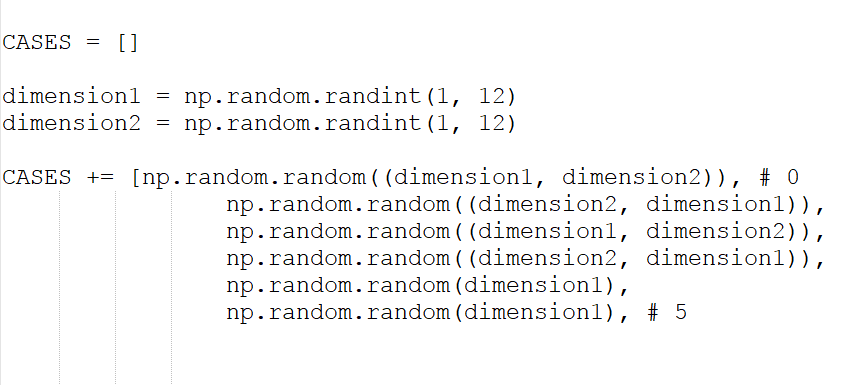
\includegraphics[width=0.70\textwidth]{snippets/multi_dot/1CASES.png}
	\includegraphics[width=0.70\textwidth]{snippets/multi_dot/2.png}
	\includegraphics[width=0.70\textwidth]{snippets/multi_dot/3.png}
	\includegraphics[width=0.70\textwidth]{snippets/multi_dot/4.png}

\end{figure}

\subsection{test\_matrix\_rank}	
\begin{figure}[h]
	\centering
	\includegraphics[width=0.70\textwidth]{snippets/rank/1.png}
\end{figure}

\subsection{test\_matrix\_determinant}	
\begin{figure}[h]
	\centering
	\includegraphics[width=0.70\textwidth]{snippets/Det/1.png}
\end{figure}

\subsection{test\_datatypes}	
\begin{figure}[h]
	\centering
	\includegraphics[width=0.70\textwidth]{snippets/datatypes/2.png}
	\includegraphics[width=0.70\textwidth]{snippets/datatypes/3.png}
	\includegraphics[width=0.70\textwidth]{snippets/datatypes/4.png}
\end{figure}

\newpage	
\end{document}
